\documentclass[a4paper,12pt,oneside]{article} 

\usepackage[utf8]{inputenc}
\usepackage[pdftex]{graphicx}
% \usepackage{polski}
\usepackage[british,UKenglish,USenglish,english,american]{babel}
\usepackage{amsfonts}
\usepackage{verbatim}
\usepackage{indentfirst}
\usepackage{listings}
\usepackage[polish]{babel}
\usepackage[T1]{fontenc}
\usepackage{fancyhdr}
\usepackage{lastpage}
\usepackage{afterpage}

\pagestyle{fancy}
\renewcommand{\headrulewidth}{0pt}
\rhead{}
\lhead{}
\cfoot{Page: \thepage/\pageref{LastPage}}

\begin{document}
\makeatletter
\addtocontents{toc}{\protect\thispagestyle{empty}}
\newcommand{\linia}{\rule{\linewidth}{0.4mm}}

\renewcommand{\maketitle}{\begin{titlepage}

    \vspace*{0.5cm}

    \begin{center}\medium

    \vspace*{0.2cm}

   Warsaw University of Technology\
\vspace{0.2cm}
    
Faculty of Electrical Engineering\\
\vspace{0.2cm}
Computer Science



    \end{center}

    \vspace*{1cm}

    \noindent\linia

    \begin{center}

      \LARGE \textsc{\@title}

         \end{center}

      \noindent\linia

    \vspace{1cm}

    \begin{flushright}

    \begin{minipage}{5cm}

    \textit{\small Authors:}\\

    \normalsize \textsc{\@author} \par

    \end{minipage}
         \end{flushright}
 \begin{center}
    \vspace{3cm}

     {\small Document done as a part of the subject:
     Python programming and data visualisation}

    \vspace*{\stretch{6}}

    \vspace{0.5cm}
    \@date

    \end{center}

  \end{titlepage}

}

\makeatother


\title{PRELIMINARY REPORT\\Project:~Python~aplication - Webservice for monitoring walking habits}

\author{Anna Głowińska\newline anna.glowinska98@gmail.com\newline index: 291070 \newline \newline
Adam Czajka\newline czajka.adam147@gmail.com \newline index: 291063}

\maketitle
\tableofcontents
\thispagestyle{fancy}
\newpage

\section{General in formations}
\subsection{Description of the application}

\textit{Monitoring walking habits} - web application that helps displaying moving routines and anomalies in moving.

\subsection{Capabilities of the application}

Application is possible to:
\begin{itemize}
\item load the data (information about the people, traces and people) from the API service,
\item present a graphs showing values of measurements for all of the sensors,
\item present the details of a single person,
\item calculate and display the details of measurements,
\item cooperate with database, which stores all of the necessary data.
\end{itemize}
\subsection{Basic concepts of the application}

The graphic user interface is shown on a graphic below.

\begin{figure}[ht]
\centering
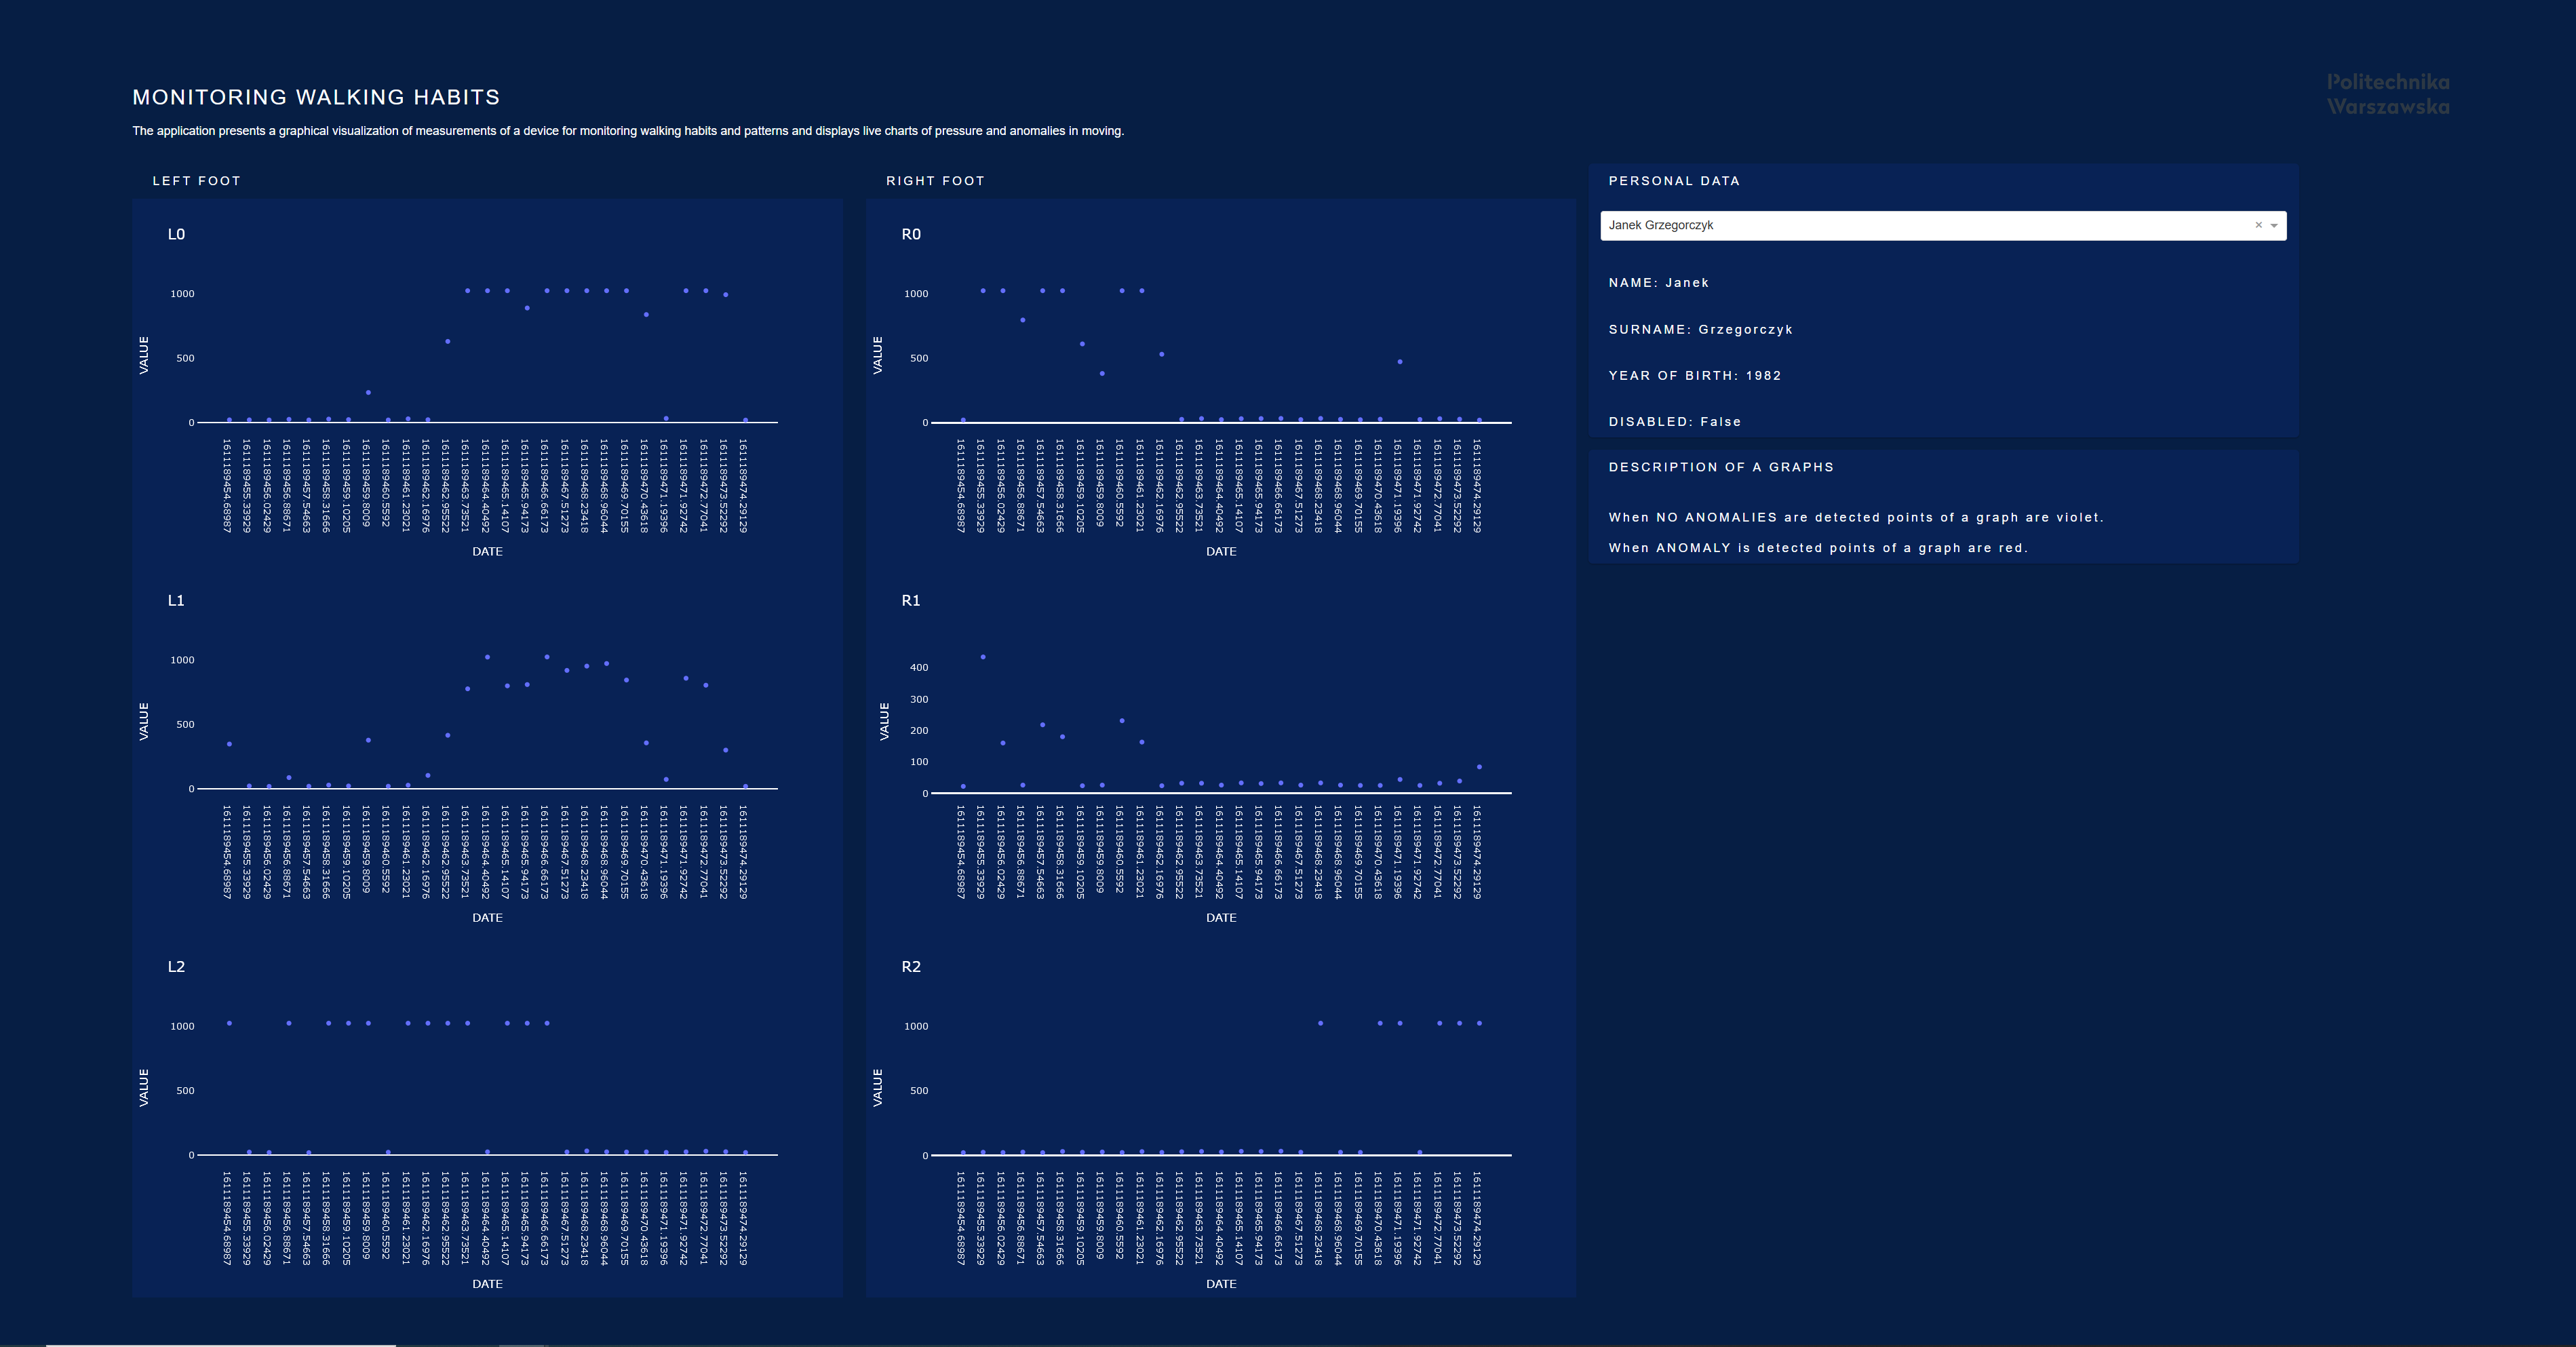
\includegraphics[width=1\textwidth]{cale.PNG}
\caption{User interface.}
\label{fig:k1}
\end{figure}

\subsubsection{Description of header}
The header shows information about the title and the main aims of an application.

\begin{figure}[ht]
\centering
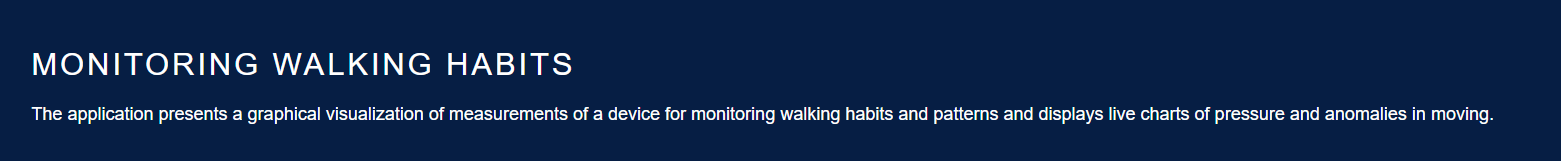
\includegraphics[width=1\textwidth]{heager.PNG}
\caption{Header.}
\label{fig:k1}
\end{figure}


\subsubsection{Description of graphs section}
Graphs show visualization of measurements of a device for monitoring walking. Graphs on the left represents sensors placed with the left foot and right - from the sensors placed with the right foot. All of the graphs are described and has animations.

\begin{figure}[ht]
\centering
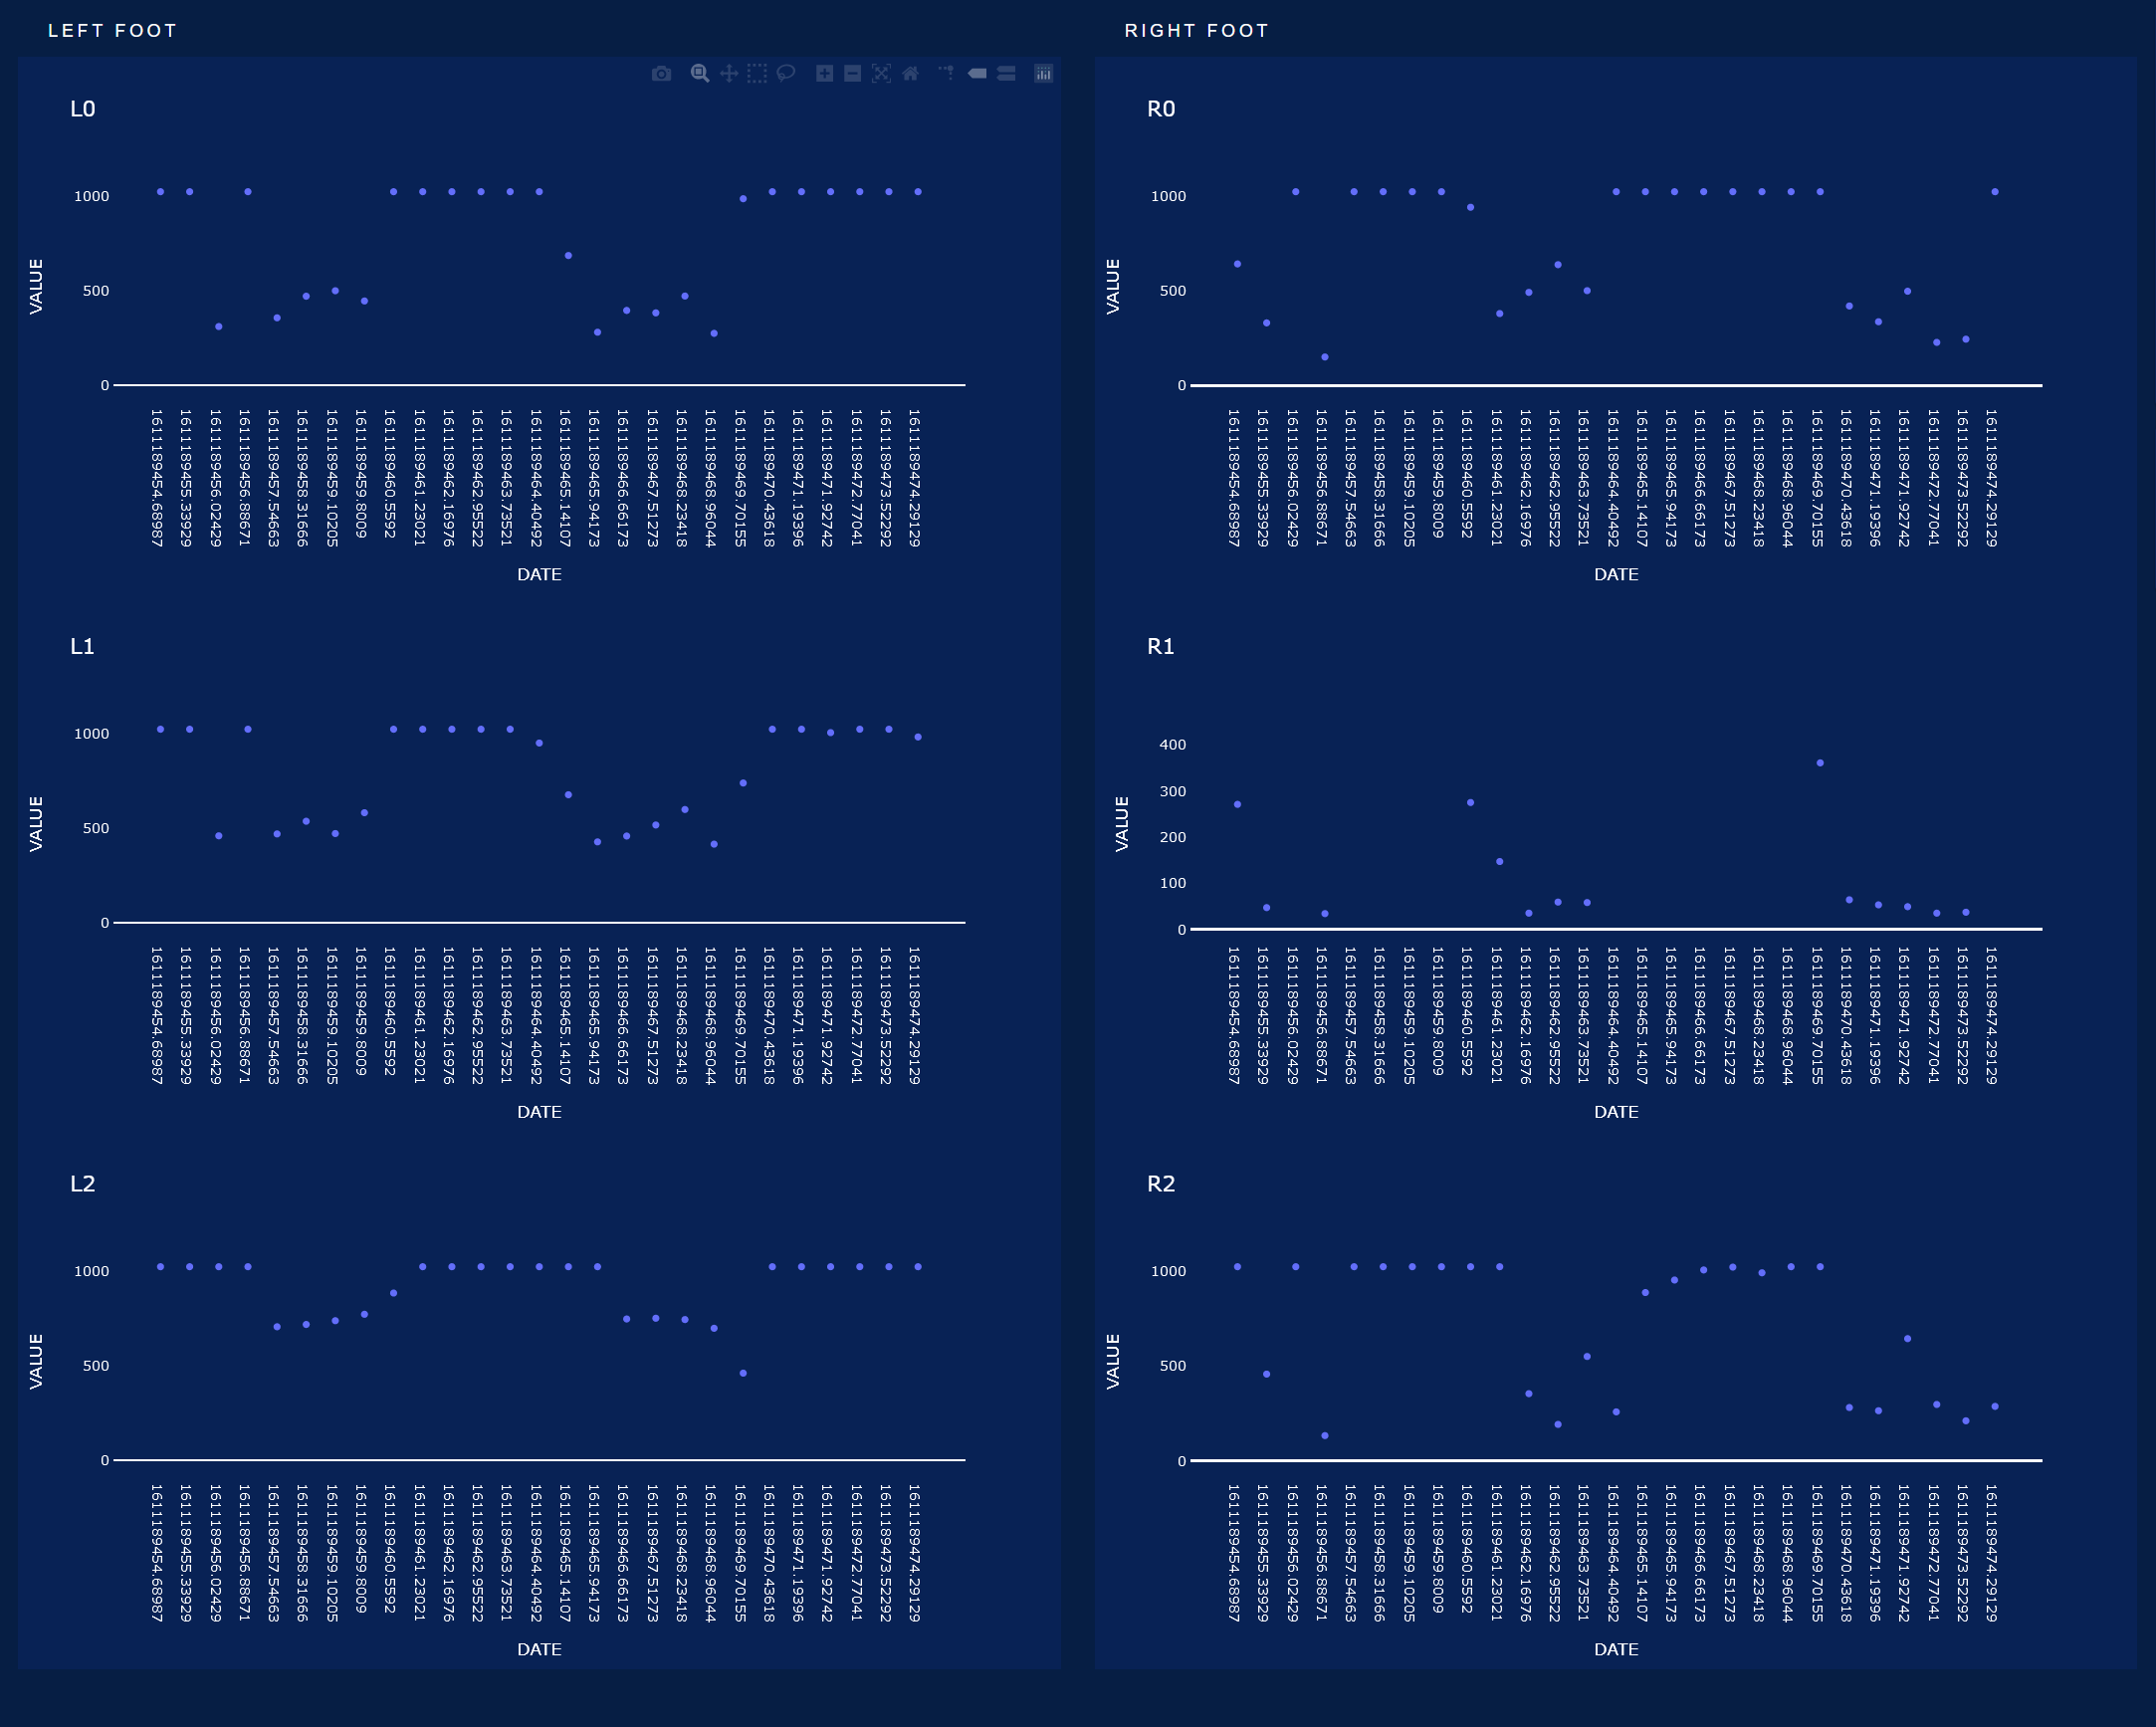
\includegraphics[width=0.8\textwidth]{wykresy.PNG}
\caption{Graphs section.}
\label{fig:k1}
\end{figure}

\newpage
\subsubsection{Description of personal data section}
This section enable user to choose a person that measurements user wants to see.
Description show more details about a single person, such as: name, surname, year of birth and if the person is disabled.

\begin{figure}[ht]
\centering
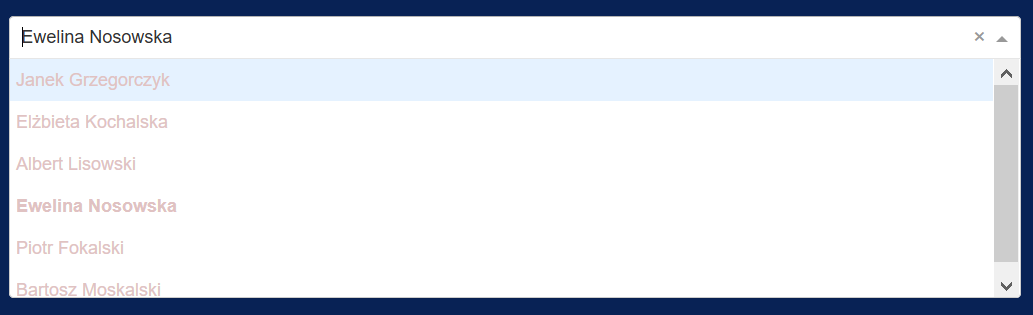
\includegraphics[width=1\textwidth]{lista.PNG}
\caption{List of people.}
\label{fig:k1}
\end{figure}

\begin{figure}[ht]
\centering
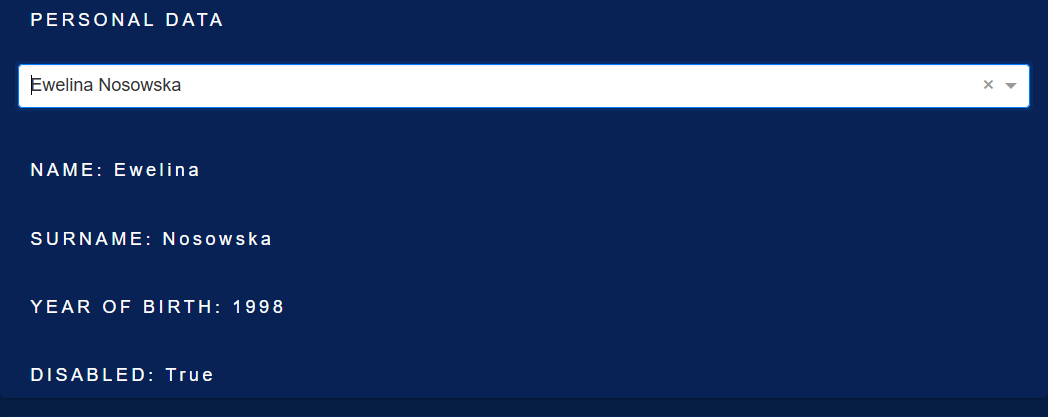
\includegraphics[width=1\textwidth]{dataper.PNG}
\caption{Personal data section.}
\label{fig:k1}
\end{figure}

\newpage
\subsubsection{Description of anomalies section}
This section presents useful information for a user, which helps to better understand the graphs - it tells when anomalies are presented on the graphs.

\begin{figure}[ht]
\centering
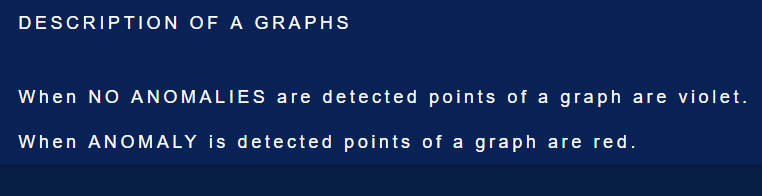
\includegraphics[width=1\textwidth]{description.PNG}
\caption{Description of anomalies.}
\label{fig:k1}
\end{figure}



\newpage
\section{Analyze of the Edward Tufte's rules}

\begin{center}
 \begin{tabular}{||c c c c||} 
 \hline
 Rule name & Importance & Percent satisfied & Explanation \\ [0.5ex] 
 \hline\hline
 Show Your Data & High & 80 & Explanation 1. \\ 
 \hline
 Use Graphics & Normal & 60 &  Explanation 2. \\
 \hline
 Avoid Chartjunk & High & 80 &  Explanation 3. \\
 \hline
 Utilize Data-ink & High & 90 &  Explanation 4. \\
 \hline
 Use Labels & High & 90 &  Explanation 5. \\ 
 \hline
 Utilize Micro/Macro & Normal & 60 &  Explanation 6. \\ 
 \hline
 Separate Layers & High & 70 &  Explanation 7. \\ 
 \hline
 Use Multiples & Normal & 75 &  Explanation 8. \\ 
 \hline
 Utilize Color & Normal & 80 &  Explanation 9. \\ 
 \hline
 Understand Narrative & Normal & 70 &  Explanation 10. \\ 
 \hline
\end{tabular}
\end{center}

Explanations:
\begin{enumerate}
    \item In the application diagrams and the data measurement work together to provide useful information.
    \item Graphs in the application are useful. 
    \item Application's data design don't focus too much on the design aspect.
    \item Application's graphs only include design elements that helps data to be understood effectively.
    \item Labels in the application are informative and essential in data design.
    \item Details of graphs and calculations in the table show better the details, what clarifies the application.
    \item All elements of the website elements have substantial differences in tone and color.
    \item Application has constancy of design. It uses many times the same type of elements of the design.
    \item The application is kept in a tone that is friendly to the user's eye. Nothing draws the eye unnecessarily, which allows you to focus on relevant information.
    \item The application follows generally accepted rules. The order in which the application elements are placed creates a logical whole.
\end{enumerate}




\section{Data format and~file structures}


\subsection{Showing anomalies}

The user is informed how to read the graphs:
\begin{itemize}
    \item when no anomalies are detected points of a graph are violet,
    \item when anomalies are detected points of a graph are red.
\end{itemize}
This situation in show on a graphic below.

\begin{figure}[ht]
\centering
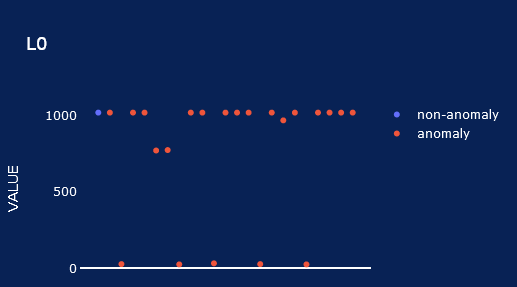
\includegraphics[width=1\textwidth]{detecAnomaly.PNG}
\caption{Detected anomalies.}
\label{fig:k1}
\end{figure}

\newpage
\subsection{Project structure}

Main concept of the project is presented in the diagram below: \newline

\par walking-monitoring
\par +--- assets
\par \ |\ \ \ \ \  +--- app.css
\par \ |\ \ \ \ \  +--- style.css
\par \ |\ \ \ \ \  +--- logo.png
\par +--- db
\par \ |\ \ \ \ \  +--- walking.db
\par \ |\ \ \ \ \  +--- db\_api.py
\par +--- app.py
\newline

Where: 
\begin{itemize}
    
\item \verb+assets+ - assets catalog,
\item  \par \verb+.css+ files - files used to styling the application,
\item \par \verb+db+ - database catalog,
\item  \par \verb+walking.db+ - database storing data,
\item  \par \verb+db_api.py+ - python file to communicate with the database,
\item  \par \verb+app.py+ - python file starting a webservice.

\end{itemize}
\subsection{Input \& output data}
\newline

All of the incoming, processed and outcoming data of the application is stored in database build in the application. When the application starts, it starts a Python process which periodically communicate with the API service and it collects the data and store it in the database. This process works on a separate thread.

\subsection{Data storage}
\textbf{SQLite Database:}
The application operates on a database \verb+walking.db+~. The database consists of three tables described below.
\newline
\par \textbf{Table people:}
Table \verb+people+ is created to store data about tested people. The table consists of the following columns: \verb+name+ , \verb+surname+ , \verb+birth_year+ , \verb+disabled+ , \verb+id+~.
\newline
\par \textbf{Table traces:}
Table \verb+traces+ is created to store data about all traces of the tested people. The table consists of the following columns: \verb+id+ , \verb+id_person+ , \verb+name+ , \verb+date+ . 
\newline
\par \textbf{Table sensors:}
Table \verb+sensors+ is created to store data about six sensors which gains information form tested people. The table consists of the following columns: \verb+id+ ,  \verb+id_trace+ ,  \verb+name+ ,  \verb+anomaly+ ,  \verb+anomaly+ ,  \verb+value+ ,  \verb+date+~.


\section{Conclusion}

The application is easy to use, the user does not have to focus on data analysis or what he has to do for the application to work properly. Graphs in the application shows data in a very ergonomic way. 
The application does not show unnecessary information, it focuses on providing the user with only relevant content.
\par Analyzing the quality of data visualization - the application satisfies the Edward Tufte's rules, both logically and visually.


\end{document}

